\chapter{Infrastructure}
\label{chap: infrastructure}

\looseness -1 \lettrine{I}{n} recent years, \muc architectures have
become the norm for server systems and are prevalent across all computing
platforms/services.  This implies server systems can exploit the inherent Instruction
Level Parallelism (ILP) of the execution flow, which is essential to improve throughput.
In addition, these processors can explore the enhanced dynamic power management (DPM)
schemes/features present to enable adequate interactiveness under power constrained
environments (e.g., mobile devices). But the paradox is that, in doing so, data centres
need to profile server systems to understand the trade-off between performance and power,
which are tightly coupled.

\nomenclature[z-ILP]{ILP}{Instruction Level Parallelism}


\looseness -1 One of the projects commissioned by the European Union FP7 and Horizon 2020
program to understand the trade-off between performance and power in both future
supercomputers and data centres is \texttt{MontBlanc}~\citep{montblanc, montblanc2,
montblancbull}.  The goal of the project is to build a ``power efficient'' server system
with multiple types of mobile cores and embedded cores~\citep{armscale}.  Specifically,
the MontBlanc prototype server at the supercomputing center in Barcelona (Spain), is
equipped with multiple boards of Samsung Exynos 5 Dual~\citep{samsung}, ARM Cortex-A15~\citep{A15}
and ARM Mali GPU T-604~\citep{Mali}. The number of clusters or servers deployed varies
depending on the demand of the data centres or supercomputers. Similarly, prior research
proposed~\citep{Halpern2016MobileSatisfaction, Wong2012KnightShift:Heterogeneity,
Chitlur2012QuickIA:Prototypes,Guevara2013NavigatingMechanisms,Mars2011HeterogeneityOpportunity,
Cong2012Energy-efficientArchitectures,DBLP:journals/ppl/VillebonnetCLPS15} several new
processors with different microarchitectural implementations, which are a direct result of
different design goals and (or) shifts in technology.

The advent of such processors allowed data centre administrators to exploit different
performance and power trade-off depending on the application requirements.  Moreover,
dynamic data centres allow more energy efficient computing services, in contrast to
stand-alone homogeneous
architectures~\citep{Mars2011HeterogeneityOpportunity}.\footnote{``Dynamic data centres''
are defined as data centres that continuously update and replace commodity servers to
improve throughput (as in Chapter~\ref{chap: REPP}).} Typically, each architecture is
categorised based the performance and power efficiency at numerous dynamic power
management features.  In this chapter, we investigate the various dynamic power management
features available, the architectures used in this thesis, the performance and power
monitoring tools used and finally the benchmarks on which the results of this thesis have
been validated on. 

\section{Dynamic Power and Performance Management} 
\label{section: Background} 

Currently available modern operating systems control the power dissipated by dynamically
controlling the power state in which the processor is at runtime.  Most operating systems,
provide an interface to monitor the processor's power state to communicate and control
with the hardware subsystem. For instance, on \textsf{Linux}, Advanced Configuration and
Power Interface (ACPI) defines a protocol to control these power states. In this section,
we give a background of the hardware settings used in this thesis.

\paragraph*{Dynamic Power Management (DPM).} DPM schemes are ingrained as an important
means to reduce power consumption in data centres having hundreds or thousands of cores,
each of them with multiple power management features. We focus on the primary DPM features
available our architectures: processor performance states (DVFS states), processor power states
(C-States), clamp states (Cl-States) and core consolidation.
DVFS states~\citep{Eric2009TheSearch, Su:2014:POP:2742155.2742200, Cochran:2011:PCA:2155620.2155641, Huang2000AManagement,Isci2006AnBudget, 6008553,  Singh2009RealCounters} and
Cl-States~\citep{Olsen:2006:PEP:1137248.1137532} have been used in numerous previous works
to provide fine-grained low-level support for a reasonable performance-power trade-off.  

\paragraph*{Processor performance states (P-States/DVFS).} Each DVFS state represents a
specified voltage and clock frequency of the cores~\citep{acpikernel} and is controlled by
the ACPI.  The frequency and voltage for
each state is described in the Differentiated System Description Table (DSDT).  The higher
numbered DVFS states correspond to higher clock frequency and higher voltage, thereby
delivering a higher performance subjected to the scalability of the workload.

The changes in DVFS state are governed using the ACPI \textsf{CPUFreq} governor using the
\textsf{acpi\_cpufreq} driver.  The default governor available using the driver as
mentioned above is \textsf{ondemand}~\citep{ondemand}, which allows the kernel to control
the core's DVFS state based on the ``load'' on the processor. However, the governor
\textit{userspace} lets users to control the core's DVFS state, via the \textsf{sysfs}
file system, manually irrespective of the ``load''.

\looseness -1 \paragraph*{Processor power states (C-States).} Modern \muc processors
support multiple C-States, also known as ``Sleep States''. These states allow various
internal modules to be turned off. Higher-numbered C-States indicate a ``deeper'' sleep
state with more internal modules disabled resulting in a lower power consumption, but
entails a longer wake up period (up to \SI{1024}{\nano\second} on an Intel machine).  At
a given C-State, all DVFS states have same power consumption when
idle~\citep{Olsen:2006:PEP:1137248.1137532}.  The choice of C-States is architecture and
processor dependent. For example, Intel Sandy Bridge supports C0, C1, C3, C6 and C7 states
and they are accessible through the \textsf{sysfs} file system, similar to the DVFS states.

\looseness -1  This technology on Intel and AMD processors is coined as
``C-States''~\citep{Intel, Schone:2015:WLP:2766527.2766547}, and on ARM processors as
``CPUidleness''~\citep{maillistperfmon}. For instance, most Intel processors support C0,
C1, C3, C6 and C7 states.  The residency period indicates the duration of time a given
core is present at a given C-State and can be controlled using the model-specific
registers (MSR).  The default time quantum for \textit{entering} a C-State is
\SI{1024}{\nano\second}.  

\paragraph*{Clamp States (Cl-States).} Although C-States are a effective power reduction
mechanisms, they are used to reduce power consumption only when the system is idle.
On the other hand, \textit{Cl-States} introduce synchronised idle injections across online
CPU threads to enable forced and controllable C-State residency.  The changes in Cl-States
are governed by ACPI using the \textsf{intel\_powerclamp} driver~\citep{powerclamp}. 


\nomenclature[z-ACPI]{ACPI}{Advanced Configuration and Power Interface}
\nomenclature[z-DSDT]{DSDT}{Differentiated State Description Table} 




\section{Architectures}
\label{sec: architecture}

In this section, we present the architectures and processors our contributions have been
evaluated. We do not enable any other internal thermal/power management algorithms which 
are run by the firmware on any processor.


\looseness -1 \paragraph*{Intel.} Intel Corei7 Sandy Bridge processor~\citep{Intel} has four
out-of-order cores enabled, each with \SI{64}{\Kilo\byte} on-chip private L1 cache and
\SI{256}{\Kilo\byte} private L2 cache. The total shared LLC was \SI{6}{\mega\byte}, and
the DRAM capacity of \SI{8}{\giga\byte} with Linux (kernel 3.14.5). The processor is
capable of DVFS from \SI{0.8}{\giga\hertz} to \SI{2.4}{\giga\hertz}.  Turbo boost and
HyperThreading were disabled.  The number of Cl-States in this study are 50 per
core.  

\looseness -1 \paragraph*{AMD.} AMD Phenom II~\citep{AMD} processor has four out-of-order
cores enabled, each with \SI{64}{\Kilo\byte} on-chip private L1 cache  and
\SI{512}{\Kilo\byte} private L2 cache.  The total shared LLC was \SI{6}{\mega\byte}, and
the DRAM capacity of \SI{8}{\giga\byte} with Linux (kernel 3.13). The processor is capable
of DVFS from \SI{0.8}{\giga\hertz} to \SI{3.2}{\giga\hertz}.  AMD processor has no
Cl-States.  

%We do not enable any other internal thermal/power management algorithms which are run by the firmware.

\begin{figure}[H] \centering
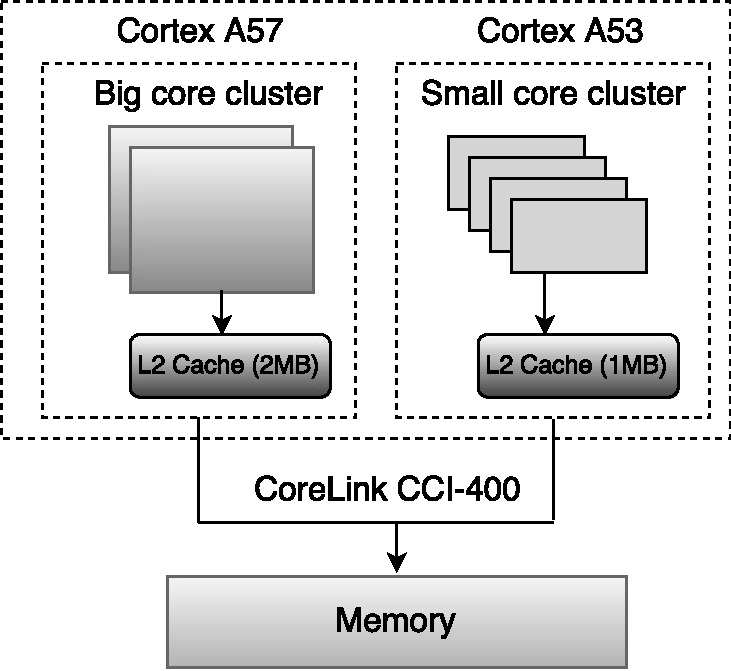
\includegraphics[width=0.4\textwidth]{Chapter2/Figs/Architecture_ARM.pdf}
\caption{Heterogeneous processor platform (ARM Juno R1)} \label{fig: archiarm}
\end{figure}

\paragraph*{ARM.} ARM Juno R1 developer board~\citep{ARM} has Linux (kernel 4.3).  The
Juno board is a \SIadj{64}{\bit} ARMv8 big.LITTLE architecture with two high-performance
out-of-order Cortex-A57 (big) cores and four low-power in-order Cortex-A53 (small) cores.
The cores are integrated on a single chip with off-chip \SI{8}{\giga\byte} DRAM.  The two
big cores form a cluster with a shared \SI{2}{\mega\byte} L2 cache, and the four small
cores form another cluster with a shared \SI{1}{\mega\byte} L2 cache.  The big cores are
capable of DVFS from \SI{0.6}{\giga\hertz} up to \SI{1.15}{\giga\hertz}, whereas the small
cores are fixed at \SI{0.65}{\giga\hertz}. The architecture is schematically shown in
Figure~\ref{fig: archiarm}. A cache coherent interconnect (CoreLink CCI-400) provides full
cache coherency among the heterogeneous cores, allowing a shared memory application to run
on both clusters simultaneously. ARM processor has no Cl-States.
    
\paragraph*{X-Gene2.} AppliedMicro X-Gene2~\citep{AppliedXGene2http://goo.gl/XA04r1} board
has Linux (kernel 4.1).  The X-Gene2 is a \SIadj{64}{\bit} homogeneous architecture with
eight out-of-order ARMv8-A cores enabled at \SI{2.4}{\giga\hertz} with
\SI{128}{\giga\byte} DRAM.  \\


In what follows, I refer to Intel Sandybridge as Intel, AMD Phenom II as AMD, and ARM Juno
R1 as ARM.


\nomenclature[z-big]{Big Core}{ARM Cortex-A57}
\nomenclature[z-small]{Small Core}{ARM Cortex-A53}

\section{Performance Monitoring} 
\label{sec: perfmon thesis}


\looseness -1 We use the performance monitoring tool,
\textsf{perf}~\citep{2016Perf:Counters}, on all architectures to gather
\textit{perf\_events}. Alternatives to \textsf{perf} include the profiling
tools (like Google wide profiler (GWP)~\citep{Ren2010Google-WideCenters, Kanev:2015:PWC:2749469.2750392}, \textsf{perfmon}~\citep{perfmon2}, etc.,) supported by
Docker, Kubernetes and LXC~\citep{Bernstein2014ContainersKubernetes}.  

\looseness -1 The ARM Juno development board raises two challenges while gathering PMCs: {\small
\circled{1}} It does not provide counters other than instructions, cache\_misses, and cycles
to be read for Cortex A53, the in-order processor, as the \texttt{CPTR\_EL3}
(Architectural Feature Trap Register) is not implemented in the Juno chip.  Therefore, the
Cortex-A53 is used only to gather basic performance statistics when throughput-oriented
workloads are collocated with interactive workloads. {\small \circled{2}} There is a known
bug~\citep{maillistperfmon} that causes \textsf{perf} to generate garbage values for all
cores whenever any core enters an idle state. Since performance statistics are only needed
when throughput-oriented workloads are run, we overcome this by disabling
CPUidle~\citep{ARMLimitedARMManual,ARMLimitedARMManualb}.  This prevents Linux from
entering the cores in an idle state when changes in the mapping cause idle periods longer
than \SI{3500}{\micro\second}.

The characterisation of workload is achieved by periodically collecting performance
statistics from the latency-critical and batch workloads. For the latency-critical
workload, we gather the appropriate ap\-pli\-cation-level QoS metrics such as throughput
(Requests Per Second -- RPS or Queries Per Second -- QPS) and latency (query tail
latency). For the batch workload, we use \textsf{perf} to characterise the thread
behaviour using the perf per thread session.


\nomenclature[z-RPS]{RPS}{Requests per Second}
\nomenclature[z-QPS]{QPS}{Queries  per Second} 

\section{Power Meters} 
\label{sec: power meters}

To gather power measurements, we use the machine's power sensor (in case of Intel and ARM)
or an external power meter (in case of AMD as power sensors are not available)
periodically during execution. The X-Gene2 board is equipped with neither a power sensor
nor attached to a power meter as it is used only as a client side request generator for
latency-critical workloads.

\looseness -1 The power meters used are as follows. {\small \circled{1}} The \textit{RAPL}
(Running Average Power Limit) register in the Intel architecture records power of core,
uncore, and DRAM controller~\citep{6008553}. The RAPL interface is accessed using the MSR
available on Intel processors~\citep{msrtool}. {\small \circled{2}} \textit{WattsUP pro}
for AMD: external device that records power of the entire system (power from
outlet)~\citep{wattsuppro}.  {\small \circled{3}} \textit{Four native energy meters} for
ARM~\citep{ARMRegisters,
ARMRegistershttps://github.com/ARM-software/devlib/blob/master/src/readenergy/readenergy.c}.
These registers report separately the power consumed by the big cluster, small cluster,
and the rest of the system (Juno's \textit{sys}
register~\citep{ARMSYS_POW_SYSHttps://goo.gl/fmTTQi}). The power consumption of the Mali
GPU is also available, but it is negligible because the GPU is disabled in all our
experiments. 

\nomenclature[z-DVFS]{DVFS}{Dynamic Voltage and Frequency Scaling}

\nomenclature[z-Cl]{Cl-States}{Idle states}
\nomenclature[z-RAPL]{RAPL}{Running Average Power Limit}
\nomenclature[z-MSR]{MSR}{Machine Specific Registers}

Table~\ref{tab:machines} summarises the architecture, processor, Linux kernel version, the
power meters, the compiler (gcc) version used for compiling the benchmarks, the range of
core frequencies (min-max) when using DVFS, the L2 and L3 cache sizes (ARM does not have
L3). The machines were available across multiple institutions (Barcelona Supercomputing
Center, University of Pittsburgh, and Universidade Federal da Bahia), and therefore we did
not have  control over the kernel and gcc versions; regardless, the results for each
architecture are consistent within that set of experiments. 

\begin{table}[t] \centering %\footnotesize \caption{\small Machines used in this study.}
    \centering
    %\footnotesize
    \caption{Machines used in this dissertation}
    \scalebox{0.84} {
        \begin{tabular}{@{}llllllllr@{}}
        \toprule
        Processor & Linux  & Power  & gcc & DFS      & L2           & L3  \\
                  & Kernel & Meter  &     & (in \SI{}{\giga\hertz}) & (size in \SI{}{\kilo\byte}) & (size in \SI{}{\mega\byte}) \\         
        \midrule

        Intel Core i7-2760QM                & 3.14.5   & RAPL                   & 4.8.1        & 0.8-2.4                & 256               & 6\\ 
            \hspace{8em}(4 cores)                                &          &                        &              &                        &                   & \\

        AMD Phenom \rom{2} X4 B97                    & 3.13.0   & WattsUp                & 4.9.2        & 0.8-3.2                & 512               & 6\\ 
                           \hspace{8em}(4 cores)                 &          & Pro                    &              &                        &                   & \\

        ARM Juno \SIadj{64}{\bit}                       & 4.3.0    & Native{\footnotesize -}                &  4.9.2       &                        &                   & no L3\\
            \hspace{2em} 2 Cortex A57                &          & energy{\footnotesize -}                &              & 0.6-1.15               & 2048              &                   \\
            \hspace{2em} 4 Cortex A53                &          & meter                  &              & 0.65                   & 1024              &\\ 
        Applied X-Gene2 \SIadj{64}{\bit}                & 4.10     & no meter               & 5.2.0        & 2.4                    & 256               & 8\\
            \hspace{8em}(8 cores)                                &          &                        &              &                        &                   & \\
        \bottomrule
    \end{tabular} }
    \label{tab:machines}
\end{table}



\section{Power Efficiency}
\label{section: power efficiency}


\looseness -1 Over the last decade, the number of services provided by data centres is increasing, and
this led to the rapid rise in the number of computing nodes. This increase in the
computational nodes raises the need to understand processors' power efficiency to maintain
and deliver the performance SLA while constrained to a strict power budget.  Moreover,
data centres spend about \SI{30}{\percent} of power allocated towards system cooling and
thereby improving the processor life time. Recent studies~\citep{4544393,
Henkel:2016:TPR:2971808.2971810, Googledatacentre, Fisher:2009:TGR:1548886.1549641} have
shown marginal rise in temperature (\SI{80}{\degree}c) is reported to reduce battery life
by \SI{50}{\percent}. Similarly, a \SI{10}{\degree}c increase in a capacitor component
temperature will reduce its life by one half~\citep{4544393}. 

For instance large-scale data centres like Facebook combat this problem in two ways:
{\small {\circled{1}}} Reducing the system cooling cost by moving to cooler climates
(\textsf{Lule\aa, Sweden}), thereby improving the power
efficiency~\citep{FBsweden}.\footnote{According to Facebook, in 2015, \textsf{Lule\aa}
warehouse was the most energy efficient data centre ever built.} {\small {\circled{2}}}
Increasing the total available power to cool the systems by using alternate sources of
fuel~\citep{FacebookHttp://goo.gl/dKVnSB}. 



\begin{table}[t]
\setlength{\tabcolsep}{1mm}
\centering
    \caption[Power and performance characterisation per architecture]{\captitle{Power and performance characterisation per architecture.} Power and performance measured using a microbenchmark on each architecture}
%\ra{1.0}
\scalebox{1}{
\begin{tabular}{@{}lrrcrr@{}}\toprule


 & \multicolumn{2}{c}{$Power\enspace (Watts)$} & \phantom{abc}& \multicolumn{2}{c}{$Perf. (\sn{IPS}{6})$}\\
\cmidrule{2-3} \cmidrule{5-6} 
Processor & All cores & One core && All cores & One core \\
\midrule
Intel                                                         &       &       &&        &       \\
    \hspace{1em}    Max frequency (\SI{2.4}{\giga\hertz})     & 27.59 & 11.67 && 19,414 & 4,822 \\
    \hspace{1em}    Min frequency (\SI{0.8}{\giga\hertz})     & 11.08 & 5.76  && 7,993  & 1,627 \\
AMD                                                           &       &       &&        &       \\
    \hspace{1em}    Max frequency (\SI{3.2}{\giga\hertz})     & 141.8 & 81.4  && 27,248 & 6,812 \\
    \hspace{1em}    Min frequency (\SI{0.8}{\giga\hertz})     & 52.8  & 48.7  && 6,786  & 1,696 \\
ARM                                                           &       &       &&        &       \\
    \hspace{1em}    Big \ \ \ A57 (\SI{1.15}{\giga\hertz})    & 2.30  & 1.62  && 4,260  & 2,138 \\
    \hspace{1em}    Small A53 (\SI{0.65}{\giga\hertz})        & 1.43  & 0.95  && 3,298  & 826   \\
\bottomrule
\end{tabular}
}
\label{tab:pphetcmp}
\end{table} 

\looseness -1 We quantify the power efficiency of our processors using the power meters
described in Section~\ref{sec: power meters} and the performance using the IPS measured
using hardware performance counters.  Table~\ref{tab:pphetcmp} summarises the power and
performance characteristics per architecture. We characterise each platform by running a
stress microbenchmark consisting of only mathematical operations without memory accesses.
For a per cluster comparison, we run the microbenchmark on all the cores in the cluster.
For a per core comparison, we run the microbenchmark on a single-core.  Specific
architectural details are as follows:

\paragraph*{Intel platform.} We characterise the homogeneous platform (four out-of-order
cores at two different frequencies). We report the power consumption obtained from the
Intel RAPL register as the sum of core, uncore and DRAM controller.  To determine the per
cluster efficiency, we run the microbenchmark on four cores at the highest and lowest
frequencies concurrently.  For the per core efficiency, we run the microbenchmark on a
single-core at the highest and lowest frequencies concurrently.

Considering the system power, a single-core at the highest DVFS state is 0.6$\times$ less
power efficient than all cores at the minimum DVFS state, in terms of IPS per watt.  This
is because, there is a minimal power consumption for the unused cores when idle and
without considering the power consumption of the idle cores, the power efficiency is
1.3$\times$.  However, taking that all cores in a cluster, and assuming that all cores are
fully utilised, four cores at the highest DVFS state is approximately (0.97$\times$) as
power efficient as four cores at the lowest DVFS state. 

\looseness -1 \paragraph*{AMD platform.} We characterise the homogeneous platform (four
out-of-order cores at two different frequencies). We report the socket power consumption
obtained from the WattsUp Pro meter.  To determine the cluster efficiency, we run the
microbenchmark on four cores at the highest and lowest frequency concurrently.  For the
per core efficiency, we run the microbenchmark on a single-core at the highest and lowest
frequency concurrently.

Considering the system power, a single-core at the highest DVFS state is 0.6$\times$ less
power efficient than all cores at the minimum frequency, in terms of IPS per watt.\ This
is because, the AMD processor does not implement C-States (or alike) to save power when
the core is idle, and therefore the single-core is not as power efficient as it could have
been.  However, taking that all cores in a cluster, and assuming that all cores are fully
utilised, four cores at the highest DVFS state are 1.5$\times$ more power efficient than
four cores at the lowest DVFS state. 

\paragraph*{ARM platform.}   We characterise the heterogeneous platform (two big cores as
big cluster, and four small cores as small cluster). We report the system power
consumption as the sum of the big and small clusters and the rest of the system (including
memory controllers, etc).  For the per-cluster comparison, we run the microbenchmark on
the big cluster and the small cluster concurrently. For a per core comparison, we run the
microbenchmark either on a single big core or on a single small core.

Considering system power, a single big core is \SI{52}{\percent}  more power efficient
than a single small core, in terms of IPS per watt. However, taking into account all cores
in a cluster, and assuming that all cores can be fully utilised, a small cluster is
\SI{25}{\percent} more power efficient than a big cluster.  This discrepancy is due to the
rest of the system, outside the core clusters, which consumes about the same power as a
big core at full utilisation (\SI{0.76}{\watt}). If we subtract the power of the rest of
the system, a single small core is $2.3\times$ more power efficient than a big core.  We
notice that small cores are attractive for throughput-oriented workloads, because of
improved power efficiency. Big cores are, however, still needed for latency-critical
workloads with tight QoS constraints, as a result of computationally-intensive
single-threaded requests.



\section{Workloads} 
\label{section: workloads}

In recent years, data centres~\citep{montblanc, Barroso2013TheEdition,
Petrucci2015Octopus-Man:Computers,Meisner2011PowerServices, Lo2015Heracles, montblanc2,
Kasture2015Rubik, montblancbull, Lo2014TowardsWorkloads} have seen an influx in a wide
range of workloads which stress different microarchitectural components.  This puts forth
the need to evaluate an algorithm for different types of workload.

We evaluated our contributions, REPP and Hipster, using throughput-oriented/batch
workloads~\citep{Mars2013Whare-map,Yang2013Bubble-flux} and interactive/latency-critical
workloads~\citep{Barroso2013TheEdition,
Petrucci2015Octopus-Man:Computers,Meisner2011PowerServices, Lo2015Heracles,
Lo2014TowardsWorkloads,Kasture2015Rubik}. These classes of workload are interesting due to
the nature of the problem they exhibit and their interactions with the hardware.  This
thesis does not explore deployment of large-scale distributed workloads, and this is left
out as future work. 


\subsection{Batch Workloads} 
\label{subsection: batch workloads}

We categorise the sequential batch workloads into single threaded batch workloads and
multiprogrammed batch workloads. For the single threaded batch workloads, we ran 22 SPEC
CPU 2006~\citep{2006core2,Henning2006SPECDescriptions}, nine PARSEC
3.0~\citep{bienia:2008:pbs:1454115.1454128}, six
NAS~\citep{Bailey:1991:NPB:125826.125925}, 11 SPLASH2x~\citep{524546}.  These workloads
exhibit both memory and computational bound phases.  The number of benchmarks in a
multiprogrammed workload, when evaluating REPP, is equal to the number of cores in each
architecture, thereby, having 35 workloads of four benchmarks on AMD and Intel, and ten
workloads of two benchmarks on ARM. When evaluating REPP, on the ARM processor, we use
only the big cluster as the small cluster does not allow us to gather most of the
counters. The methodology to build the workloads is described by Sanchez and
Kozyrakis~\citep{Sanchez:2011:VSE:2000064.2000073}.

The benchmarks are divided into four categories, following the categorisation by Sanchez
and Kozyrakis~\citep{Sanchez:2011:VSE:2000064.2000073}. We run all the applications in
isolation and gather PMCs at a sampling frequency of \SI{250}{\milli\second} until the
end, and compute mean value of the ratio of number of kilo-IPS to kilo-LLC misses. For
all workloads, we select the native input set size.  Those which have  ratio less 0.1 are
considered as Thrashing or Streaming (\textbf{S}), applications that benefit cache size,
that is, ratio between 0.1 and 0.2 are classified as Cache-Fitting (\textbf{T}).  Then,
applications with a ratio between than 0.2 and 1 are classified as Cache-Friendly
(\textbf{F}). Finally, applications with ratio greater than 1 are classified as
Insensitive (\textbf{N}). There are 35 possible combinations (with repetitions) of these
four categories, each of which forms a group. In the multiprogrammed workloads consisting
of four benchmarks (on Intel and AMD) from SPEC, PARSEC 3.0, NAS, and SPLASH2x suites, we
have one mix per group.  In the multiprogrammed workloads, each application is randomly
selected from the category.  This results in 35 workloads.  The same methodology is
followed on ARM, where there are 10 possible combinations (with repetitions) of these four
categories, each of which forms a group. In those multiprogrammed workloads consisting of
two benchmarks from PARSEC 3.0, NAS, and SPLASH2x, we have one mix per group. Note that
SPEC could not be compiled on ARM.  Table~\ref{tab: classes} shows the categorisation of
the workloads.  This technique of selecting multiprogrammed workloads facilitates for
significant difference in the size of the shared memory footprint and number of stall
cycles of the processor. Tables~\ref{tab: classes-ARM} and~\ref{tab: classes-AMD-Intel}
show the multiprogrammed workloads on ARM, AMD and Intel.  

The threads in a multiprogrammed workload run continuously until the longest thread in
execution finishes (other threads restart execution immediately as they finish).  To
ensure statistically significant results, we ran each workload multiple times and had a
\SI{95}{\percent} confidence with a very low error margin (less than \SI{2}{\percent}).
In the graphs that follow, we do not show the error margin to avoid visual clutter.  


\nomenclature[a-N]{$N$}{Insensitive batch workload} 
\nomenclature[a-F]{$F$}{Cache Friendly batch workload} 
\nomenclature[a-T]{$T$}{Cache Fitting batch workload} 
\nomenclature[a-S]{$S$}{Thrashing batch workload}



\subsection{Latency-Critical Workloads} 


\looseness -1 We evaluate the effectiveness of Hipster using two latency-critical
workloads, Memcached~\citep{MemcachedHttps://memcached.org/}, and
Web-Search~\citep{Elasticsearchhttps://github.com/elastic/elasticsearch}, which have
distinct characteristics and impact on shared resources~\citep{Lo2015Heracles}.
\textbf{Memcached}~\citep{MemcachedHttps://memcached.org/} is an open source
implementation of an in-memory key-value store for data caching used in many services from
Twitter, Facebook and Google~\citep{199376,
Nishtala2013ScalingFacebook,Atikoglu2012WorkloadStore}.  The backend of
\textbf{Web-Search}~\citep{Barroso2003WebArchitecture, JanapaReddi2010WebCores, 199376} is
an instance of
Elasticsearch~\citep{Elasticsearchhttps://github.com/elastic/elasticsearch}, an open
source implementation of a search engine used by many companies including Netflix and
Facebook.  The load generator (Faban~\citep{FabanHttp://faban.org/}) for Memcached and
Web-Search is adapted from CloudSuite 3.0~\citep{Ferdman2012ClearingClouds}. It is
configured to model diurnal load changes, simulating a period of
36~hours~\citep{Meisner2011PowerServices}; each hour in the original workload corresponds
to one minute in our experiments.

\looseness -1 We also evaluate the effectiveness of Hipster by collocating a single
interactive workload, and a mix of batch workloads. The objective of the collocation is to
maximise the throughput of the batch workloads while satisfying QoS of the interactive
workload. The number of batch workloads is equal to the number of cores not utilised by
the interactive workload. We report the system throughput by aggregating the IPS of all
batch programs.

\looseness -1 When implementing Hipster, the ARM processor is used when collocating a
latency-critical workload with a batch workload, and running a latency-critical workload in
isolation; The workload generator runs on another machine: XGene2.


\begin{table}[t]
    \centering
    %\setlength{\tabcolsep}{3.5pt}
	%\caption{Workload configurations, maximum load while meeting the target tail latency with two big cores for latency-critical applications.}
    \caption[Latency-critical workload configuration]{\captitle{Latency-critical workload configuration.} Workload configurations, maximum load while meeting the target tail latency with two big cores.} 
    %for latency-critical applications.}
	\scalebox{1}{
    \begin{tabular}{@{}llllr@{}}
        \toprule
        App & Workload  	& Max. Load & Target Tail \\
        	& Configuration	&			 & latency (ms) \\
        \midrule
        Memcached  & Twitter caching       & 36\,000\,RPS & 10 (95\%ile)\\
                   & server of \SI{1.3}{\giga\byte}       & 		   &   				\\
        Web-Search & English Wikipedia     & 44\,QPS | think-    & 500 (90\%ile)\\
        		   & Zipfian distribution  & time of 2sec\citep{FabanHttp://faban.org/}&				\\
        \bottomrule
    \end{tabular}
    }   
    \label{tab:configs}
\end{table}


\paragraph*{Assessment metric for latency-critical applications.} Quality of Service for
social-networking sites like Twitter and Google require fast rendering of user-content
with strict SLA requirements such as requests per second. In addition, to statistically
compute the average latency, QoS often focuses on tail latency which is defined as the
upper bound of latencies experienced by \ninefive or \ninenine percentile of flows (for
example, TCP flows, HTTP requests, RPCs, etc.) to improve
interactivity~\citep{Dean2013TheScale}.

\paragraph{Tail latency requirements.} For Memcached, we define the tail latency to be the
\ninefive percentile request latency, with a target of
\SI{10}{\milli\second}~\citep{Lo2014TowardsWorkloads,Ferdman2012ClearingClouds}; for
Web-Search, we define it to be the \ninezero percentile query latency, with a target of
\SI{500}{\milli\second}~\citep{Ferdman2012ClearingClouds}. The load for Memcached and
Web-Search are measured in terms RPS and QPS, respectively.  Table~\ref{tab:configs} lists
the two latency-critical applications, their configurations, maximum loads, and target
tail latency in milliseconds. For each latency-critical workload, the maximum load is
chosen so that the platform is able to meet the tail latency when running on the big cores
at maximum DVFS.


\nomenclature[z-QoS]{QoS}{Quality of Service} 

\nomenclature[z-IPS]{IPS}{Instructions Per Second}

\nomenclature[z-LLC]{LLC}{Last Level Cache}

\section{Conclusion} \label{section: chap2conclusion}  

In this chapter, we have introduced the architectures, the power meters, the performance
monitoring tools, the type of workloads our results have been evaluated on. In a nutshell,
the work has been carried out on three \SIadj{64}{\bit} architectures: Intel SandyBridge,
AMD Phenom \rom{2}, and ARM Juno. Each of these architectures is equipped with a power
meter to gather power statistics. Similarly, we install a performance monitoring tool to
gather performance statistics per application.  Finally, the single threaded workloads are
taken from four different benchmark suites: SPEC CPU 2006, PARSEC, SPLASH, and NAS. The
multiprogrammed workloads were designed based on the methodology described by Sanchez and
Kozyrakis~\citep{Sanchez:2011:VSE:2000064.2000073}.



%%%%%%%%%%%%%%%%%%


\iffalse
\begin{table*}[htb]
    \centering
    \caption{Categorisation of workloads.}
    \scalebox{0.95}{
        \begin{tabular}{lllllr}
        \toprule 
            Label & Description   & Intel-Benchmarks & AMD-Benchmarks                                        & ARM-Benchmarks \\
        \midrule 
            N & Insensitive       & bzip2, blackscholes, bodytrack,    & blackscholes, bzip2, calculix, ep.C, & blackscholes, ep.C, fft \\
            &                   & calculix, dedup, ep.C, freqmine,     & facesim, freqmine, gobmk, gromacs,   & fluidanimate, freqmine \\ 
            &                   & gobmk, gromacs, h264ref, hmmer,      & h264ref, hmmer, is.C, lu\_cb, namd,  & is.C, lu\_cb,lu\_ncb \\ 
            &                   & is.C, lu\_cb, namd, omnetpp,         & omnetpp, povray, radiosity, raytrace, &    \\ 
            &                   & povray, raytrace, tonto, vips        & raytrace, sjeng, tonto, volrend        & \\ 
            &                   &                                      & water\_nsquared, water\_spatial       &\\ 
            F   & Cache Friendly    & cactusADM, cg.C, lbm, libquantum & bodytrack, cactusADM, canneal, cg.C  & facesim, radiosity  \\ 
                &                   & lu\_ncb, ocean\_cp, sjeng        &            fmm, lu\_ncb, ocean\_cp, streamcluster    & streamcluster,volrend\\ 
                &                   & water\_spatial, x264, zeusmp     & vips, wrf, x264,
                zeusmp          & water\_nsquared\\ 

        T & Cache Fitting     & astar, bwaves, canneal, gemsFDTD                    & astar, bwaves, dedup, radix                           & canneal, radix, raytrace, vips\\
          &                   & radix, soplex                                       & soplex                                                &  water\_spatial\\

        S & Thrashing         & lu.C, mcf, milc, mg.C, sp.C                         & gemsFDTD, lbm, libquantum, lu.C                       & bodytrack, cg.C, dedup, fmm\\
          &                   & streamcluster, xalancbmk                            & mcf, mg.C, milc, sp.C, xalancbmk                      & lu.C, mg.C, ocrean\_cp, sp.C\\

        \bottomrule
        \end{tabular} 
    }
    \label{tab: classes}
\end{table*}
\fi 


\iffalse
\begin{landscape}

\begin{table}[htb]
    \centering
%\setlength{\tabcolsep}{1pt}
    \caption[Categorisation of workload]{\captitle{Categorisation of workloads based on methodology described in~\citep{Sanchez:2011:VSE:2000064.2000073}.} The label, and description for each benchmark from SPEC, NAS, PARSEC, and SPLASH2x. The labels are read as follows: N as Insensitive, F as Cache-Friendly, T as Cache-Fitting, and S as Streaming/Thrashing}    
    \scalebox{0.95}{
    \begin{tabular}{@{}ll ccc  
                       ll ccc c@{}}
        \toprule 
        & & \multicolumn{3}{c}{$Platform$} & & & \multicolumn{3}{c}{$Platform$} \\
        \cmidrule{3-5} \cmidrule{8-10} 
        $Benchmark$ & $Suite$ & $Intel$ & $AMD$ & $ARM$ & $Benchmark$ & $Suite$ & $Intel$ & $AMD$ & $ARM$ \\
        \midrule
        Bzip2       & SPEC    & N       & N     & -  & Barnes      & SPLASH2x& F       & T     & T \\
        Calculix    & SPEC    & N       & N     & -  & Fft         & SPLASH2x& N       & N     & N \\
        Gobmk       & SPEC    & N       & N     & -  & Fmm         & SPLASH2x& F       & F     & S \\
        Gromacs     & SPEC    & N       & N     & -  & lu\_cb      & SPLASH2x& N       & N     & N \\
        H264ref     & SPEC    & N       & N     & -  & lu\_ncb     & SPLASH2x& F       & F     & N \\
        Hmmer       & SPEC    & N       & N     & -  & ocean\_cp   & SPLASH2x& F       & F     & T \\

        Namd        & SPEC    & N       & N     & -  & Radix       & SPLASH2x& T       & T     & T \\
        Omnetpp     & SPEC    & N       & N     & -  & Volrend     & SPLASH2x& N       & N     & F \\
        Povray      & SPEC    & N       & N     & -  &Water\_nsquared& SPLASH2x& N       & N     & F \\
        Tonto       & SPEC    & N       & N     & -  & Blackscholes& PARSEC  & N       & N     & N \\
        CactusADM   & SPEC    & F       & F     & -  & Bodytrack   & PARSEC  & N       & F     & S \\
        Lbm         & SPEC    & F       & S     & -  & Dedup       & PARSEC  & N       & T     & S \\
        Libquantum  & SPEC    & F       & S     & -  & Canneal     & PARSEC  & T       & F     & T \\
                                                     
        Sjeng       & SPEC    & F       & N     & -  & Facesim     & PARSEC  & N       & N     & F \\
        Zeusmp      & SPEC    & F       & F     & -  & Fluidanimate& PARSEC  & N       & N     & N \\
        Wrf         & SPEC    & F       & F     & -  & Freqmine    & PARSEC  & N       & N     & N \\                                                  
        Astar       & SPEC    & T       & T     & -  & Raytrace    & PARSEC  & N       & N     & T \\
        Bwaves      & SPEC    & T       & T     & -  & Streamcluster& PARSEC  & S       & S     & F \\
        Soplex      & SPEC    & T       & T     & -  & Vips        & PARSEC  & N       & F     & T \\
        GemsFDTD    & SPEC    & T       & S     & -  & x264        & PARSEC  & F       & F     & T \\
        Mcf         & SPEC    & S       & S     & -  & ep.C        & NAS     & N       & N     & N \\
        Milc        & SPEC    & S       & S     & -  & is.C        & NAS     & N       & N     & N \\
        Xalancbmk   & SPEC    & S       & S     & -  & cg.C        & NAS     & F       & F     & S \\
        Radiosity   & SPLASH2x& N       & N     & F  & lu.C        & NAS     & S       & S     & S \\  
        Raytrace    & SPLASH2x& N       & N     & T  & mg.C        & NAS     & S       & S     & S \\  
        Water\_spatial& SPLASH2x& F       & N     & T& sp.C        & NAS     & S       & S     & S \\  

        \bottomrule
        \end{tabular}
    }
    \label{tab: classes}
\end{table}

\end{landscape} 
\fi



\begin{landscape}

\begin{table}[htb]
    \centering
%\setlength{\tabcolsep}{1pt}
    \caption[Categorisation of workload]{\captitle{Categorisation of workloads based on methodology described in~\citep{Sanchez:2011:VSE:2000064.2000073}.} The label, and description for each benchmark from SPEC, NAS, PARSEC, and SPLASH2x. The labels are read as follows: N as Insensitive, F as Cache-Friendly, T as Cache-Fitting, and S as Streaming/Thrashing}    
    \scalebox{0.90}{
        \begin{tabular}{@{}ll ccc c@{}}  
        \toprule 
        & & \multicolumn{3}{c}{$Platform$}  \\
                \cmidrule{3-5}             
        $Benchmark$ & $Suite$ & $Intel$ & $AMD$ & $ARM$ \\
        \midrule
        Bzip2       & SPEC    & N       & N     & -  \\   
        Calculix    & SPEC    & N       & N     & -  \\   
        Gobmk       & SPEC    & N       & N     & -  \\   
        Gromacs     & SPEC    & N       & N     & -  \\   
        H264ref     & SPEC    & N       & N     & -  \\   
        Hmmer       & SPEC    & N       & N     & -  \\   
                                                       
        Namd        & SPEC    & N       & N     & -  \\   
        Omnetpp     & SPEC    & N       & N     & -  \\   
        Povray      & SPEC    & N       & N     & -  \\   
        Tonto       & SPEC    & N       & N     & -  \\   
        CactusADM   & SPEC    & F       & F     & -  \\   
        Lbm         & SPEC    & F       & S     & -  \\   
        Libquantum  & SPEC    & F       & S     & -  \\   
                                                       
        Sjeng       & SPEC    & F       & N     & -  \\   
        Zeusmp      & SPEC    & F       & F     & -  \\   
        Wrf         & SPEC    & F       & F     & -  \\   
        Astar       & SPEC    & T       & T     & -  \\   
        Bwaves      & SPEC    & T       & T     & -  \\   
        Soplex      & SPEC    & T       & T     & -  \\   
        GemsFDTD    & SPEC    & T       & S     & -  \\   
        Mcf         & SPEC    & S       & S     & -  \\   
        Milc        & SPEC    & S       & S     & -  \\   
        Xalancbmk   & SPEC    & S       & S     & -  \\   
        Radiosity   & SPLASH2x& N       & N     & F  \\   
        Raytrace    & SPLASH2x& N       & N     & T  \\   
        Water\_spatial& SPLASH2x& F       & N     & T\\   

        \bottomrule
        \end{tabular}
        \hspace{1em}
        \begin{tabular}{@{}ll ccc c@{}}  
        \toprule 
        & & \multicolumn{3}{c}{$Platform$}  \\
                \cmidrule{3-5}             
            $Benchmark$ & $Suite$ & $Intel$ & $AMD$ & $ARM$  \\
            \midrule
                                                                                                       
             Barnes      & SPLASH2x& F       & T     & T \\
             Fft         & SPLASH2x& N       & N     & N \\                                                 
             Fmm         & SPLASH2x& F       & F     & S \\                                                  
             lu\_cb      & SPLASH2x& N       & N     & N \\
             lu\_ncb     & SPLASH2x& F       & F     & N \\                                                  
             ocean\_cp   & SPLASH2x& F       & F     & T \\
                                                                                                              
             Radix       & SPLASH2x& T       & T     & T \\
             Volrend     & SPLASH2x& N       & N     & F \\
            Water\_nsquared& SPLASH2x& N     & N     & F \\
             Blackscholes& PARSEC  & N       & N     & N \\
             Bodytrack   & PARSEC  & N       & F     & S \\
             Dedup       & PARSEC  & N       & T     & S \\
             Canneal     & PARSEC  & T       & F     & T \\
                                                                                                              
             Facesim     & PARSEC  & N       & N     & F \\
             Fluidanimate& PARSEC  & N       & N     & N \\
             Freqmine    & PARSEC  & N       & N     & N \\                                                  
             Raytrace    & PARSEC  & N       & N     & T \\
            Streamcluster& PARSEC  & S      & S     & F \\
             Vips        & PARSEC  & N       & F     & T \\
             x264        & PARSEC  & F       & F     & T \\
             ep.C        & NAS     & N       & N     & N \\
             is.C        & NAS     & N       & N     & N \\
             cg.C        & NAS     & F       & F     & S \\
             lu.C        & NAS     & S       & S     & S \\  
             mg.C        & NAS     & S       & S     & S \\  
             sp.C        & NAS     & S       & S     & S \\  

        \bottomrule
        \end{tabular}
    }
    \label{tab: classes}
    \end{table}
\end{landscape} 

